\section{Fenômenos de Transporte de Calor}

A transferência de calor é um fenômeno em que, na física, dois corpos com temperaturas diferentes trocam suas energias térmicas quando estão em contato ou em um mesmo ambiente, para que atinjam o equilíbrio.

Alguns materiais são isolantes térmicos e tendem a evitar transferência. São importantes para prevenir gasto energético desnecessário e manter sistemas sem troca de calor se necessário.

Para o projeto proposto, é necessário uma temperatura interna entre 2 e 4 graus Celsius para preservar as características desejadas e não danificar o órgão colocado. Além disso, a caixa deve ser isolada termicamente para que minimize ao máximo as trocas de calor e não afete o órgão transportado.

Essa transferência de calor pode ser classificada de três formas diferentes: Condução, convecção e radiação.

\subsection{Condução}
Ocorre entre corpos que estão em contato físico e está relacionada com a energia cinética, a colisão entre os átomos realiza a transferência de energia cinética (calor) para as moléculas próximas. Com isso, o calor flui do local com temperaturas mais altas para o local com temperatura mais baixa.

A facilidade com que o calor transferido pode ser medido através da condutividade, normalmente, sólidos conduzem melhor que líquidos, e líquidos conduzem melhor do que sólidos.

\begin{table}[H]
\centering
\begin{tabular}{|c|c|}
\cline{1-2}
Material               & Condutibilidade Térmica (k) \\ \cline{1-2}
Cobre (puro)           & 339                         \\ \cline{1-2}
Ouro (puro)            & 317                         \\ \cline{1-2}
Alumínio (puro)        & 237                         \\ \cline{1-2}
Ferro (puro)           & 80,2                        \\ \cline{1-2}
Aço Carbono (1\%)      & 43                          \\ \cline{1-2}
Aço Inoxidável (18/18) & 15,1                        \\ \cline{1-2}
Vidro                  & 0,81                        \\ \cline{1-2}
Plásticos              & 0,2 -- 0,3                  \\ \cline{1-2}
Água (liquido)         & 0,6                         \\ \cline{1-2}

\end{tabular}
\caption{Condutividade térmica dos materiais a 300K. Fonte: BENNETT, 2008}
\label{condutividade térmica}
\end{table}

\subsection{Convecção}

A convecção ocorre em líquidos ou gases somente. Ocorre pela diferença de densidades, o ar frio é mais denso e tom ao lugar do ar quente, o ar frio lentamente ganha calor e realiza o ciclo novamente.

Existem dois tipos de convecção: a natural (explicada acima) e a forçada, a qual utiliza aspiradores e bombas para fazer o deslocamento do fluído. (BENNETT, 2008; TIPLER, 2009).

\subsection{Radiação}

São ondas eletromagnéticas que se movem na velocidade da luz, por ser a única capaz de percorrer o espaço, é a principal maneira de transferência de calor do Sol com o planeta terra.

\begin{figure}[H]
\centering
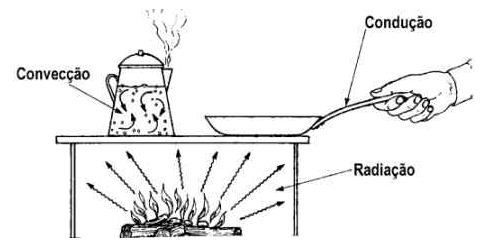
\includegraphics[width=8cm]{figuras/transferenciadecalor.png}
\caption{Mecanismos de transferência de calor}
\end{figure}

\section{Calorimetria}
A calorimetria é o estudo do calor como energia térmica em trânsito. Com dois corpos em temperaturas diferentes, a transmissão ocorre do corpo mais quente para o mais frio até atingirem o equilíbrio térmico. Uma das medidas mais usadas é a quantidade de calor (Q), ao receber energia térmica, essa quantidade de calor é positiva, ao perder é negativa.

\subsection{Calor Sensível e Latente}
Um corpo pode receber dois tipos de calor, o latente e o sensível. O calor latente é obtido quando o corpo muda de estado físico por causa dessa transferência, já o calor sensível é apenas mudança na temperatura do corpo.

Podemos representar seus cálculos com a fórmula fundamental da calorimetria e a equação para calcular o calor latente. Que são:

\begin{align}
Q_S=m \cdot c \cdot \Delta T
\end{align}
\begin{align}
Q_L=m \cdot L
\end{align}

Onde:
\begin{itemize}
\item $Q_S$ = Quantidade de calor sensível (em joules)
\item m = Massa do corpo em gramas
\item c = Calor sensível
\item $\Delta$T = Diferença de temperatura em ºC
\item $Q_L$ = Quantidade de calor Latente (em joules)
\item L = Constante de calor latente
\end{itemize}

